\documentclass{svproc}

\usepackage{url}
\def\UrlFont{\rmfamily}

\usepackage{makecell}

\usepackage{graphicx}

\usepackage{subcaption}
\captionsetup{compatibility=false}

\usepackage[utf8]{inputenc}
\usepackage[T1]{fontenc}

% for \textdegree symbol
\usepackage{textcomp}

% comments on the margin
\usepackage{todonotes}

\begin{document}
\mainmatter

\title{The utilization of spherical camera in simulation for service robotics}
%\titlerunning{}

\author{Krystian Chachuła \and Maciej Stefańczyk}
%\authorrunning{}
%\tocauthor{}

\institute{
    Warsaw University of Technology,\\Institute of Control and Computation Engineering\\
Nowowiejska 15/19, 00-665 Warsaw, Poland\\
\email{krystian.chachula.stud@pw.edu.pl} \\
\email{maciej.stefanczyk@pw.edu.pl}
}

\maketitle

\begin{abstract}

    Safety is one of the most important factors in robotics, especially when robots have to 
    collaborate with people in common environment. Testing the physical systems, however, must
    focus on much more than just a software. One of the common steps in robotic system development
    is utilization of simulators, which are very good for tasks like navigation or manipulation.
    Testing vision systems is more challenging, as the simulated data often is far from the
    real camera readings. In this paper, we show the advantages of using the spherical camera
    for recording the sequences of test images and a way to integrate those with existing
    robotic simulator. The presented system has also the possibility to be extended with rendered
    objects to further improve its usability.

% A set of spherical images can be used to obtain photorealistic images from a simulated regular camera.
% The position of such virtual camera determines the spherical image that is being used for image generation.
% Its orientation along with camera parameters is used to transform a spherical image to a regular image.
% Software implementing this method of simulation has been integrated into the Robot Operating System framework and the Gazebo simulator. This integration allows users to use this solution in existing projects without much overhead.
% Moreover, Gazebo integration makes it possible to overlay virtual objects onto virtual camera images.

\keywords{spherical camera, service robotics, robot simulation, ROS}
\end{abstract}

\section{Introduction}

\subsection{The problem}

People use their sight as the most important sense when they move through their surroundings.
It is therefore essential for service robots to use image processing.
When robots coexist with humans, safety is highly important \cite{haddadin2007safety}.
One of many measures to be taken is software testing,
which requires test data and, in the domain of computer vision, this data consists of images or videos from a robot's camera \cite{7759425}.
However, using a real robot for testing can be dangerous.
The danger stems from the fact that, while testing, the robot is controlled by yet untested software, which, in case of service robots, can be complicated \cite{Dudek-multitasking-romoco-2019-twiki}. This can lead to damaging the environment, the robot itself or in the worst case scenario can harm the people.
Using a real robot for testing can also be tedious -- after each test iteration one has to return the environment to the initial state and move robot back to the staring pose.
To speed up the process it is possible to run the application on multiple robots \cite{levine2018learning}, but this is not the cost-effective solution.
This creates the need to simulate the tested robot and, specifically, its one or more cameras.

\subsection{State of the art}
An effective method of gathering image data for testing is recording a video while the robot is executing a given path in the testing environment for future use.
Another way is using simulators such as Gazebo \cite{koenig2004design} or UnrealROX \cite{martinez2019unrealrox}.
Gazebo is meant to be an universal simulator, with physics and 3D rendering engine. It allows for accurate 
robots and environment modelling and robots behavior simulation. Its integration with the Robot Operating \
System makes it very popular amongst the research and industry community. It is lacking the most in the vision 
field. Although the 3D rendering is possible, environments created in the simulation are often filled
with repetitive objects with very simple textures (fig.~\ref{fig:gazebo_vs_real}).
 Lighting system is also very simplified, withouth any 
shadows and reflections, which makes the renders unsuitable for the vision algorithms evaluation. 

\begin{figure}[!ht]
    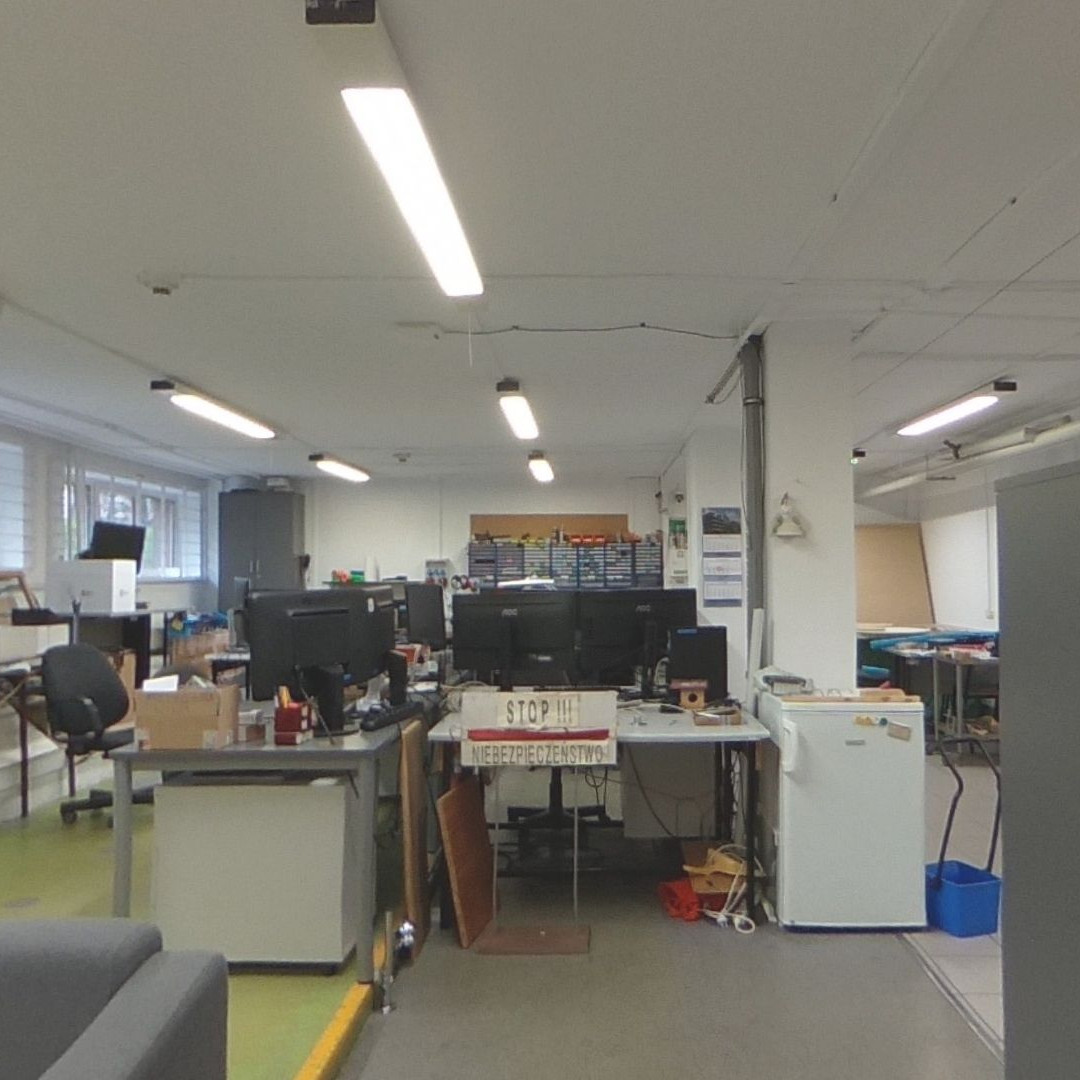
\includegraphics[width=0.485\textwidth]{img/gazebo_vs_real/real.jpg}\hfill%
    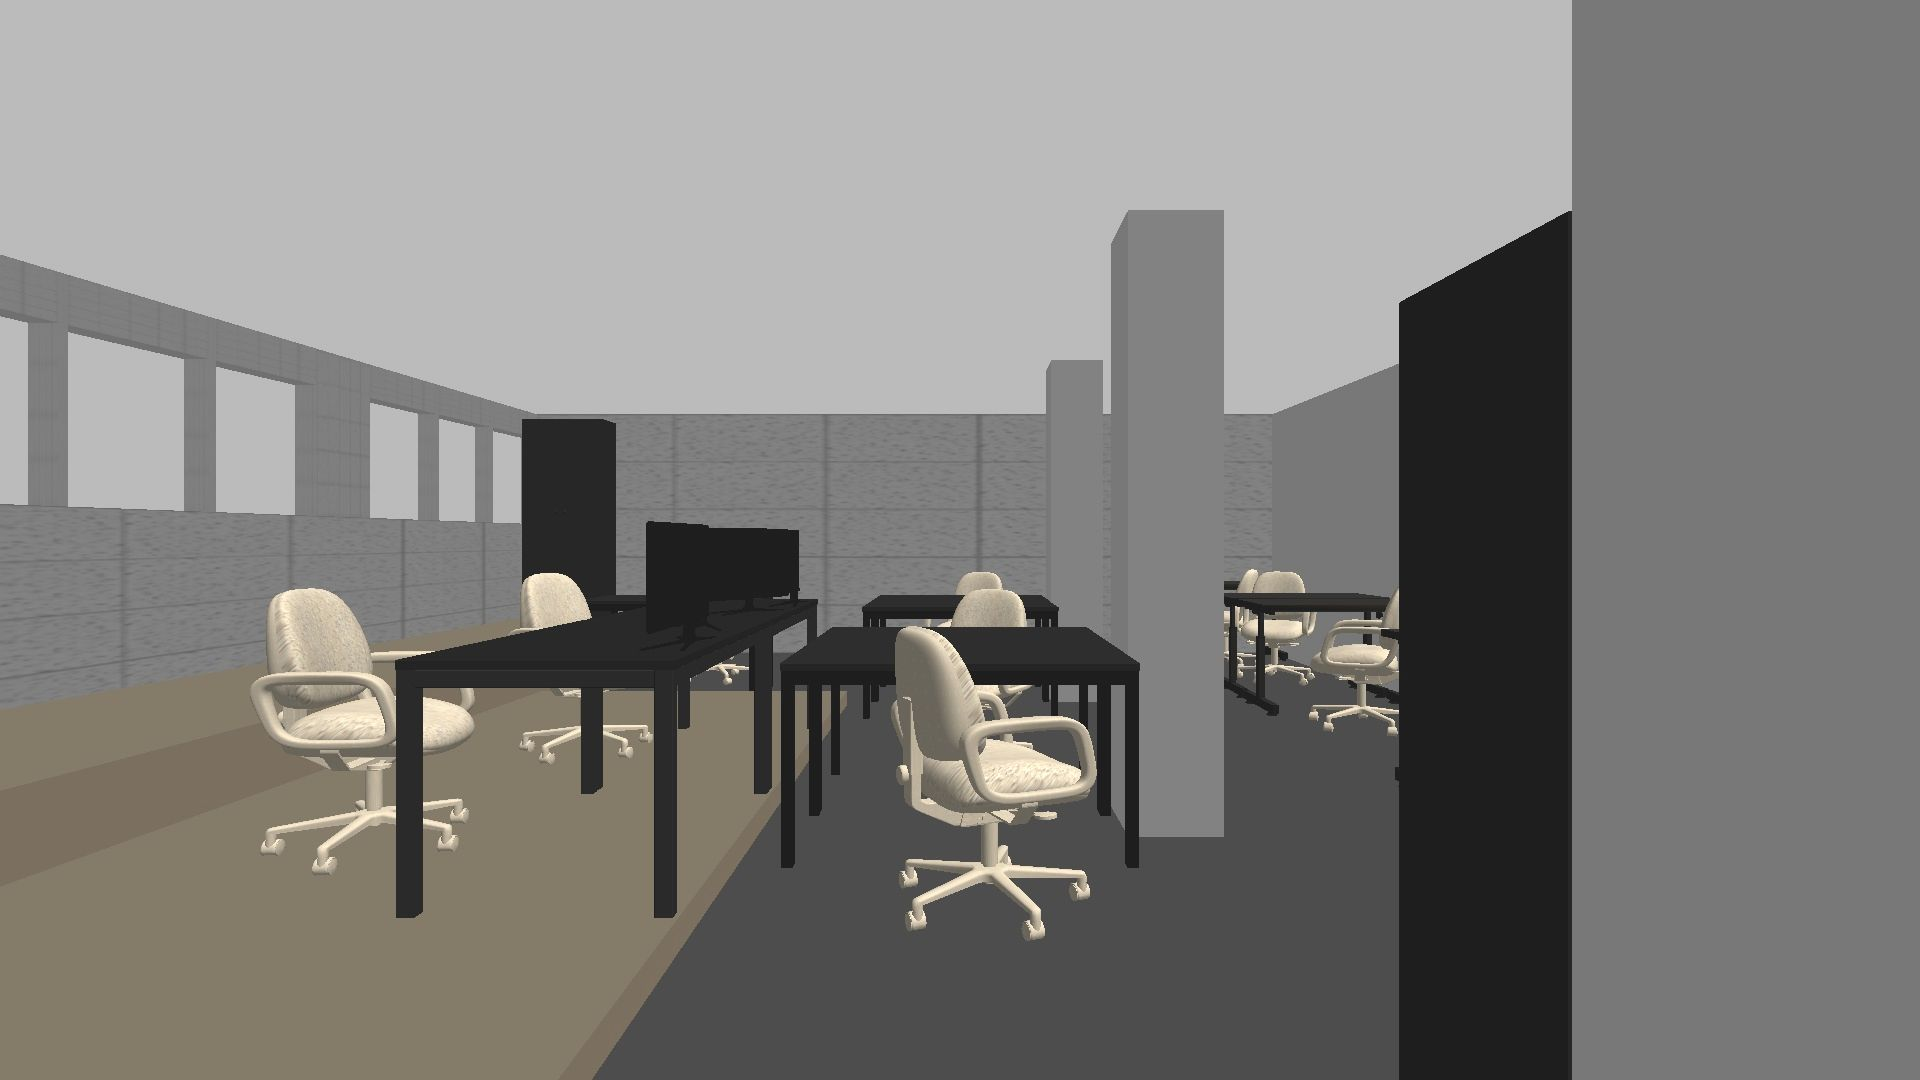
\includegraphics[width=0.485\linewidth]{img/gazebo_vs_real/gazebo.jpg}
    \caption{A real (left) and a simulated (right) camera in Gazebo}
    \label{fig:gazebo_vs_real}
\end{figure}\vspace{-1mm}

On the other hand, simulators like UnrealROX are designed to be used as a tool for training visual algorithms,
especially those based on deep learning, requiring a lot of training data. Simulator, based on Unreal Engine, 
is able to produce photorealistic scenes in realtime (fig.~\ref{fig:rox_samples}). To prepare such scenes, 
however, an artist is required most of the time. Solution like this would be perfect, but lack of integration 
(and no possibility thereof) with robotics systems makes it a tool only for offline learning, not interactive
testing.

\begin{figure}[!htb]
    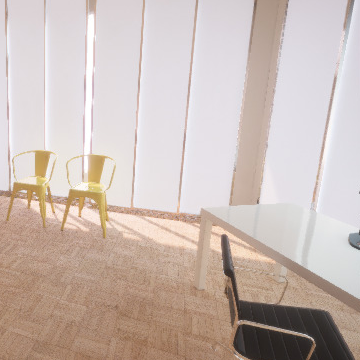
\includegraphics[width=0.485\textwidth]{img/gazebo_vs_real/rox1.png}\hfill%
    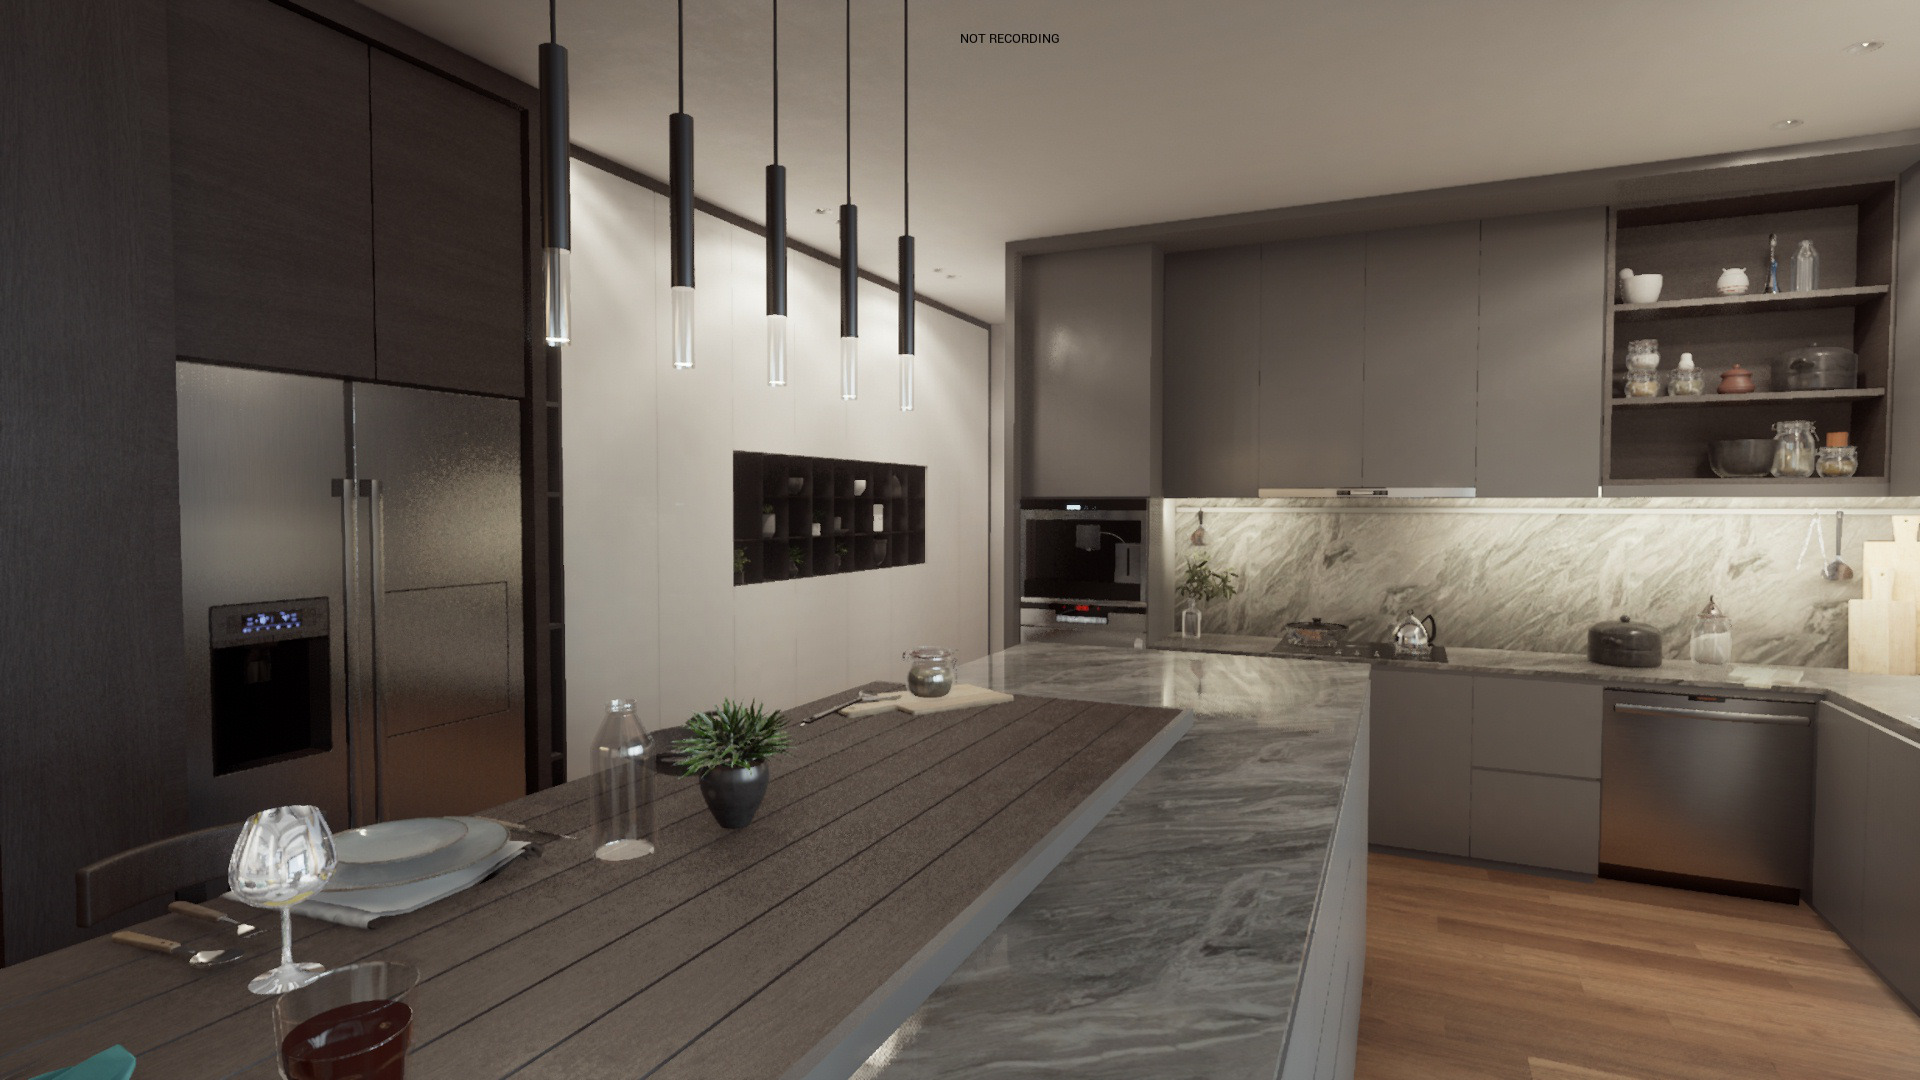
\includegraphics[width=0.485\linewidth]{img/gazebo_vs_real/rox2.png}
    \caption{Sample images generated by the UnrealROX simulator \cite{martinez2019unrealrox}}
    \label{fig:rox_samples}
\end{figure}

From this short review we can point out some features that are desired in simulators \cite{staranowicz2011survey} 
apart from the photorealism.
One is the capability to quickly modify the world model used for image generation.
This allows the tester to create new test scenarios rapidly.
Another important feature is the ability to dynamically edit the robot's path.
Of course this is not possible when simulating using a prerecorded video, but should be achievable 
in every generic simulator, as well as the capability of simulating robot's interactions with the
environment, such as collisions and manipulation. Integration with ROS is also important. From the summary
in tab.~\ref{tab:simulation_methods} we can see, that fulfilling all the requirements at once is hard to achieve.

\begin{table}[!ht]
    \centering
    \setlength{\tabcolsep}{1em}
    \def\arraystretch{1.2}
    \begin{tabular}{ |c|c|c|c|c| } 
        \hline
        Feature & \textit{Gazebo} & \makecell{\textit{Pre-recorded} \\ \textit{video}} & \textit{UnrealROX} \\ 
        \hline
        \makecell{environment modification} & yes & \textbf{no} & yes \\
     %   \hline
        \makecell{editable robot path} & yes & \textbf{no} & yes \\
     %   \hline
        \makecell{interaction with the environment} & yes & \textbf{no} & yes \\
     %   \hline
        photorealism & \textbf{no} & yes & yes \\
     %   \hline
        ROS integration & yes & yes & \textbf{no} \\
        \hline
    \end{tabular}
        \vspace*{1em}
        \caption{Comparison of different camera simulation methods}
        \label{tab:simulation_methods}
\end{table}\vspace{-5mm}

\subsection{The solution}

Using prerecorded video/images has the biggest photorealism (as those are photos). Using the 3D simulators gives 
possibility of free robot movement and interaction with the environment. As a way to combine both worlds
we study the possibility of using the photos as a source for the camera image in the simulation. 
To give the robot possibility to look around photos should cover full sphere (360\textdegree\ panorama or 
full spherical photo). To have freedom of movement images from (almost) all possible robot locations should 
be available. The position of the virtual camera can be used to select exactly one (the closest) spherical image from the set.
Finally, to not limit the solution to only single pre-recorded environemnt state, there has to be
a way of adding the simulated/rendered objects to the scenes. This will also allow for interaction. Schematic
diagram of proposed system is presented on fig.~\ref{fig:flow}.

The rest of the paper is structured as follows. In section~\ref{sec:spherical} we show the methods of creating
a single photo from a spherical image. Following section introduces a way of dealing with robot movement.
Integration with Gazebo simulator and merging with the rendered overlays is presented in section~\ref{sec:gazebo}.
A case study for a prepared system is presented in section~\ref{sec:evaluation}, followed by the conlusions.

\begin{figure}[ht!]
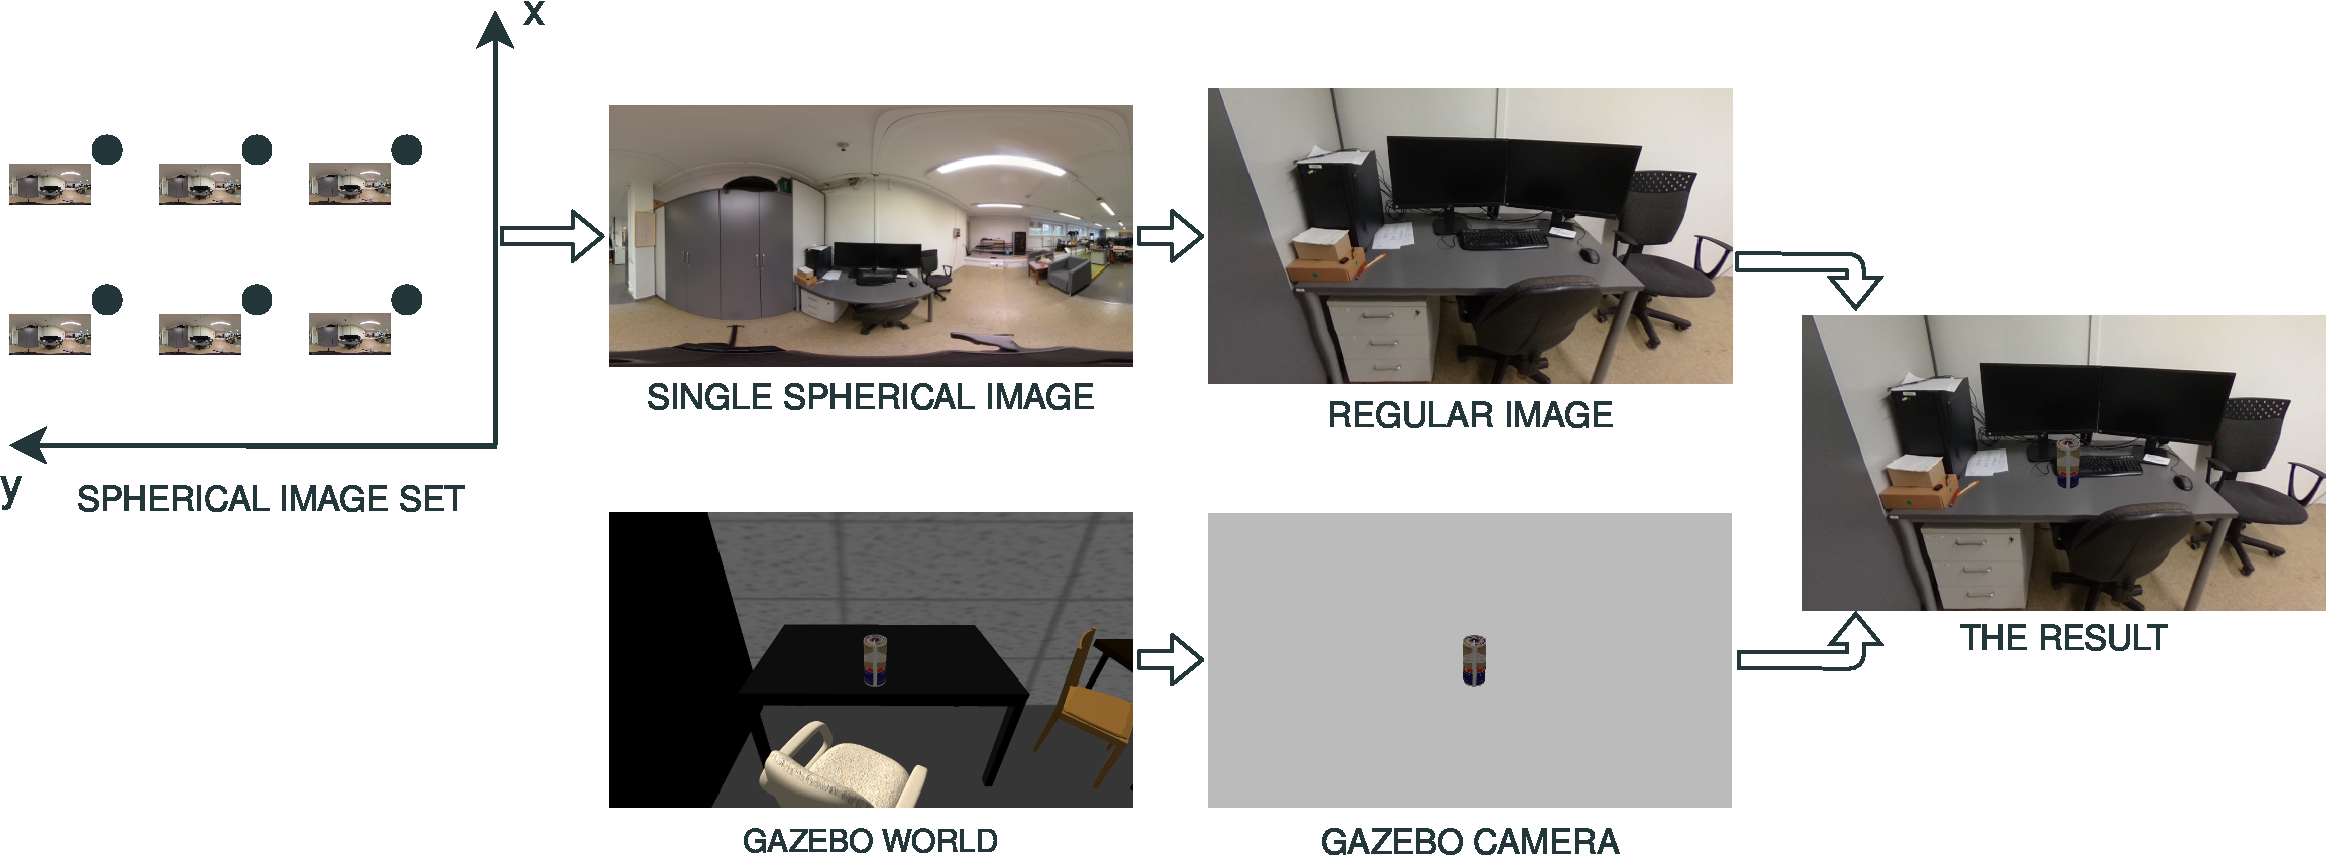
\includegraphics[width=\textwidth]{img/drawio/flow.pdf}
\caption{Schematic diagram of proposed simulation system}
\label{fig:flow}
\end{figure}

% Images from a spherical camera can be used to photorealistically simulate an environment.
% The idea is visualized on Fig. \ref{fig:flow}.

% First a set of spherical images is needed.
% The images are tagged with the position where each of them was taken.
% The position of the virtual camera can be used to select exactly one (the closest) spherical image from the set.
% A single spherical image can be transformed into a regular image using the virtual camera orientation and virtual camera parameters.
% \begin{figure}[!ht]
%     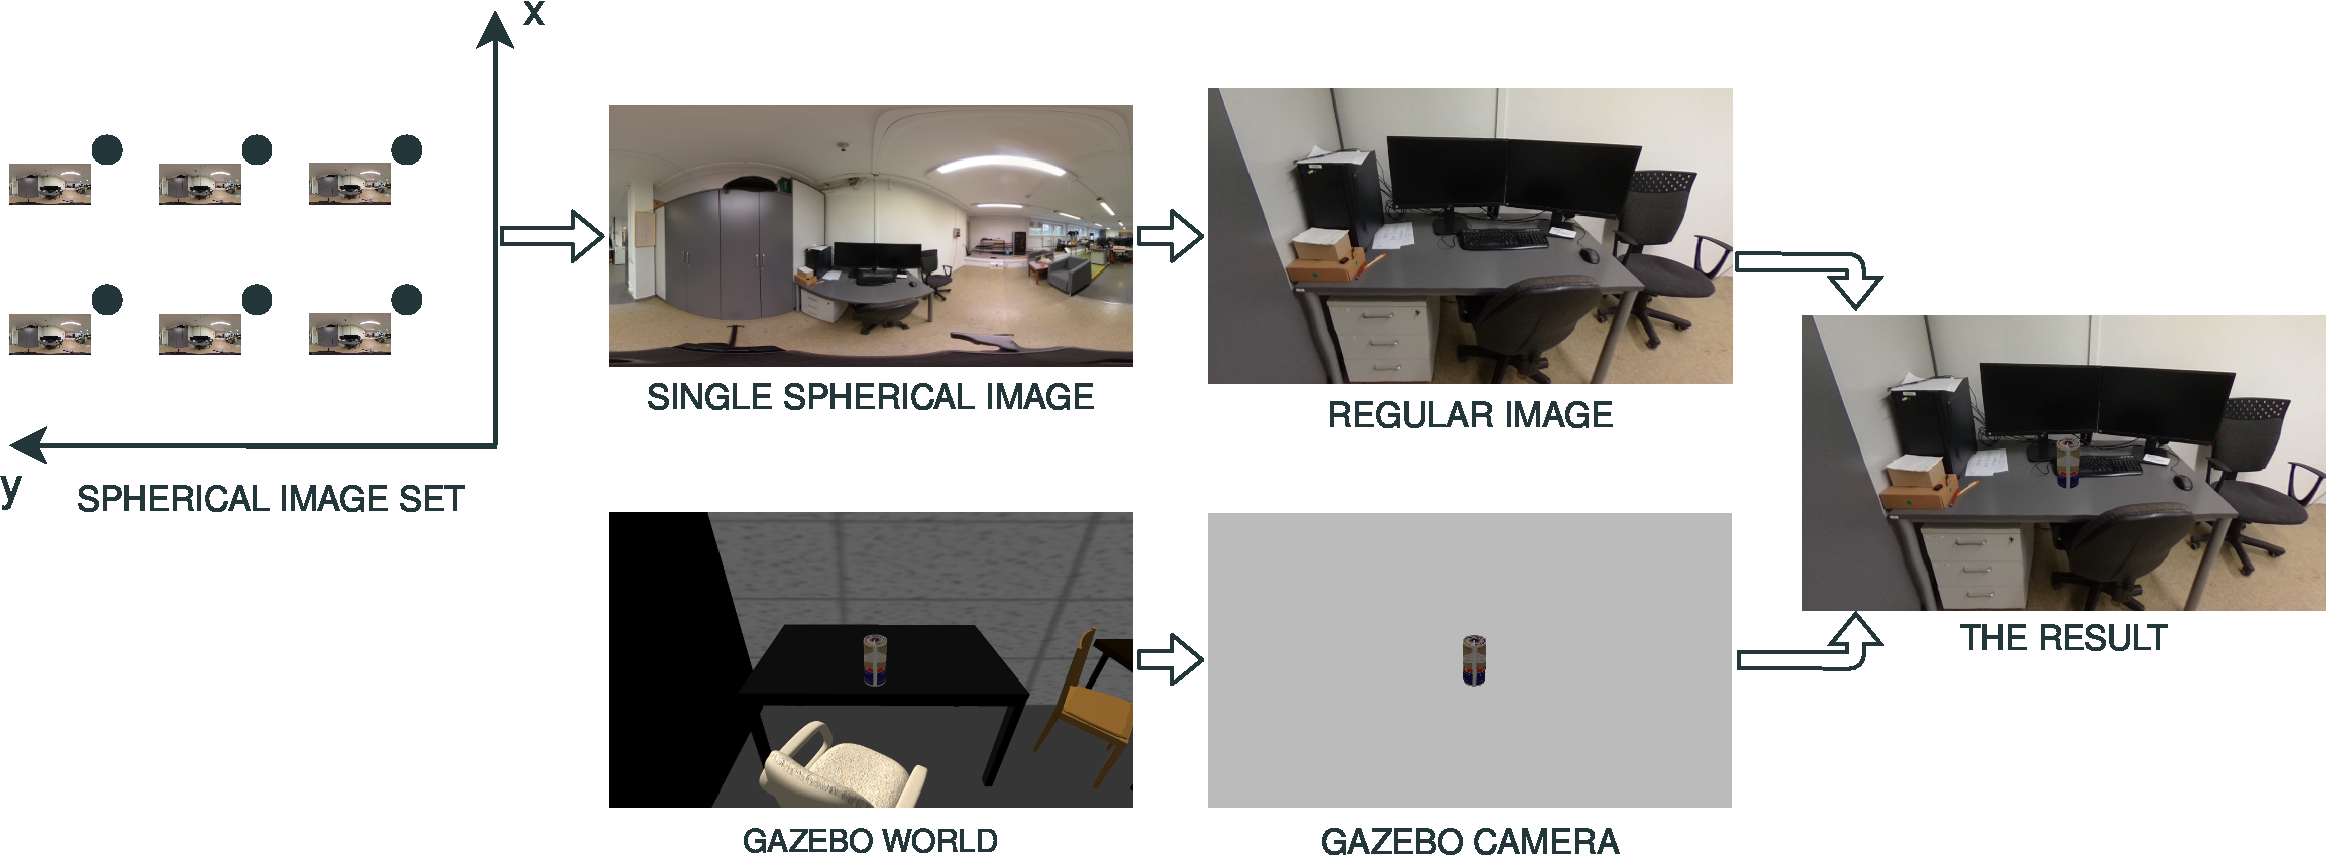
\includegraphics[width=\textwidth]{img/drawio/flow.pdf}
%     \caption{The idea of the system}
%     \label{fig:flow}
% \end{figure}

%\subsection{Nomenclature}

There are different camera types used throgh the article. A \textbf{spherical camera} is a type of camera with a field of view that covers the entire sphere and a \textbf{regular camera} is a type of camera with a field of view close to $90$ degrees.
The camera that belongs to a robot in sumulation is referred to as a \textbf{virtual camera}.
A \textbf{projection camera} is an entity that projects a 3D scene to a 2D image in computer graphics.




\section{Transforming spherical images}
\label{sec:spherical}

In order to transform a spherical image to a regular image one can utilize 3D computer graphics.
Not only is this method simple, but its implementation can utilize hardware acceleration unlike other solutions. \footnote{https://github.com/scihant/CTPanoramaView} \footnote{https://github.com/mistic100/Photo-Sphere-Viewer} \footnote{https://github.com/bingsyslab/360projection} \footnote{https://github.com/fuenwang/Equirec2Perspec} 

A sphere is a 3D closed surface where every point on the sphere is the same distance from its origin.
% The equation of a sphere with center at point $(x_0, y_0, z_0)$ and radius $R$ is as follows:
% \begin{equation}
%     (x - x_0)^2 + (y - y_0)^2 + (z - z_0)^2 = R^2
% \end{equation}
Since only a finite number of points can be drawn, a sphere will need to be approximated by drawing a subset of its points.
Those points can be selected by creating a UV Sphere.
A UV Sphere consists of vertices that are created by performing angular steps in the spherical coordinate system (fig.~\ref{fig:spheres}a).
Cartesian points are generated using these equations:
\begin{equation}
    x = R \cdot \cos \phi \cdot \cos \theta \quad y = R \cdot \cos \phi \cdot \sin \theta \quad z = R \cdot \sin \phi \nonumber
\end{equation}
where $R$ is the radius of the sphere, $\phi \in [0, \pi]$ -- polar angle and $\theta \in [0, 2\pi)$ -- azimuthal angle.

Then the sphere has to be textured with the spherical image (fig.~\ref{fig:spheres}b).
Most spherical cameras create images in the form of equirectangular projections, and, without the loss
of generality of the solution, we assumed images in that format are available.
The process of texturing a UV sphere with an image in the form of this projection is fairly straightforward \cite{greene1986environment}. 
Every point on the sphere can be mapped to a point on the texture using the following equations:
% \begin{eqnarray}
%     x_t &=& R(\theta - \varphi_0) \cos \phi_1 \nonumber \\
%     y_t &=& R(\phi - \theta_1)
% \end{eqnarray}
% where $\theta_0$, $\phi_1$ -- center coordinates.
% Those equations can be simplified by assuming $\theta_0 = 0$ and $\phi_1 = 0$.
% The sphere can also be assumed to be normalized ($R = 1$), which further simplifies the equations.
\begin{equation}
    x_t = \theta \nonumber \quad y_t = \phi
\end{equation}

Having textured the sphere, now a projection camera can be placed in its center (fig.~\ref{fig:spheres}c).
Its parameters (field of view and resolution) are set to match the robot's virtual camera.
The image from this camera is a regular image as seen by the robot looking in given direction.

\begin{figure}[ht!]
    \centering
    a) \hspace{-3mm}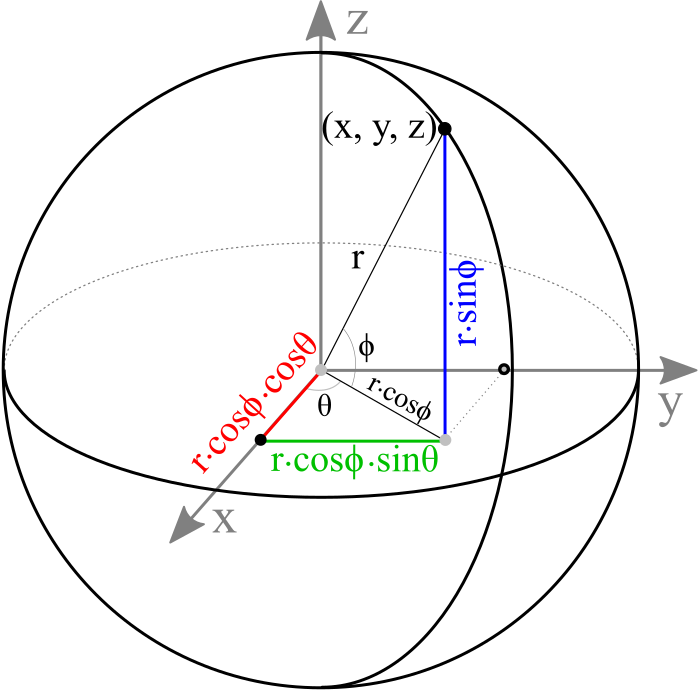
\includegraphics[width=0.32\textwidth]{img/genpoint}
    b) \hspace{-3mm}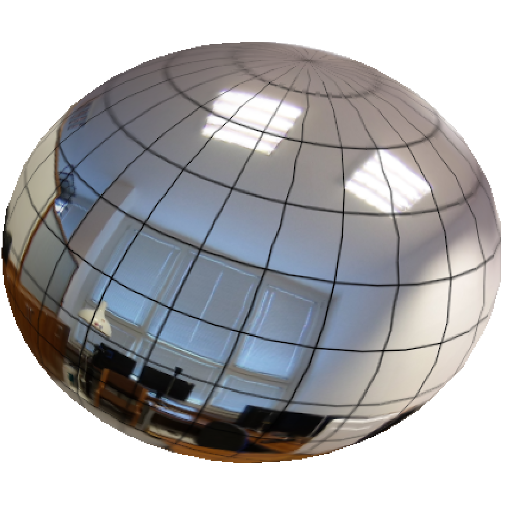
\includegraphics[width=0.32\textwidth]{img/gl_sphere/textured}
    c) \hspace{-3mm}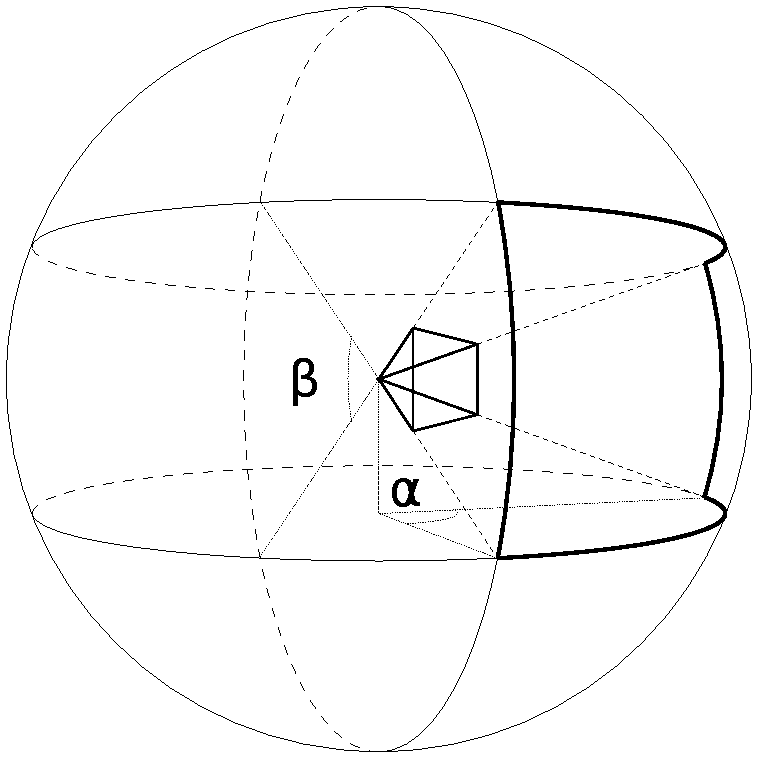
\includegraphics[width=0.32\textwidth]{img/sphere}
    \caption{Creating regular image from the spherical photo}
    \label{fig:spheres}
\end{figure}

\section{Interpolation}
\label{sec:iterpolate}


The fact that always the nearest spherical image is used for rendering poses a significant issue.
This problem is visualized on Fig.~\ref{fig:interpolation}a.
The dots represent the set of spherical images (top-down view) and the grid divides the surface into regions tied to a spherical image at its center.
Camera icons symbolize exemplary positions and orientations of virtual cameras with equal parameters.
All cameras use the same spherical image for simulation (the closest image is marked orange).
Moreover, all cameras have the same orientation relative to the global reference frame.
This means that the same regular image would be produced for all the cameras.

\begin{figure}[!ht]
    \centering
    a) 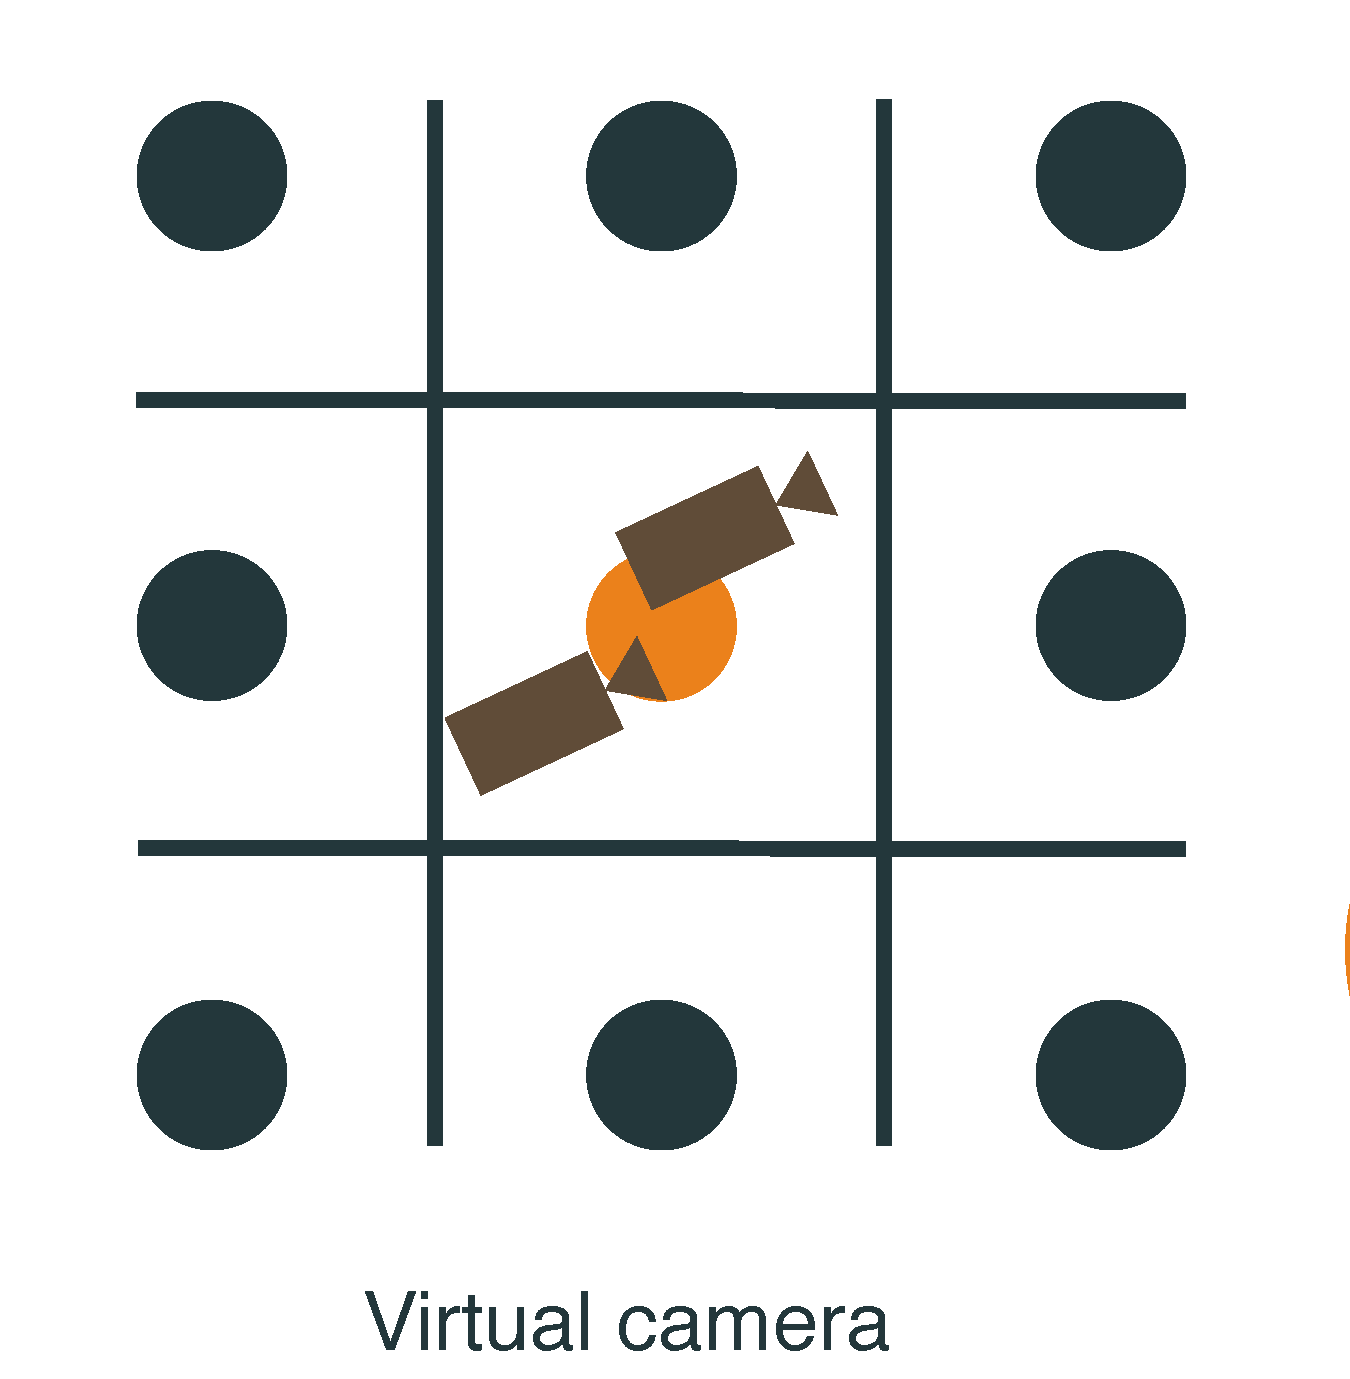
\includegraphics[width=0.45\textwidth]{img/interpolation/virt.pdf}
    b) 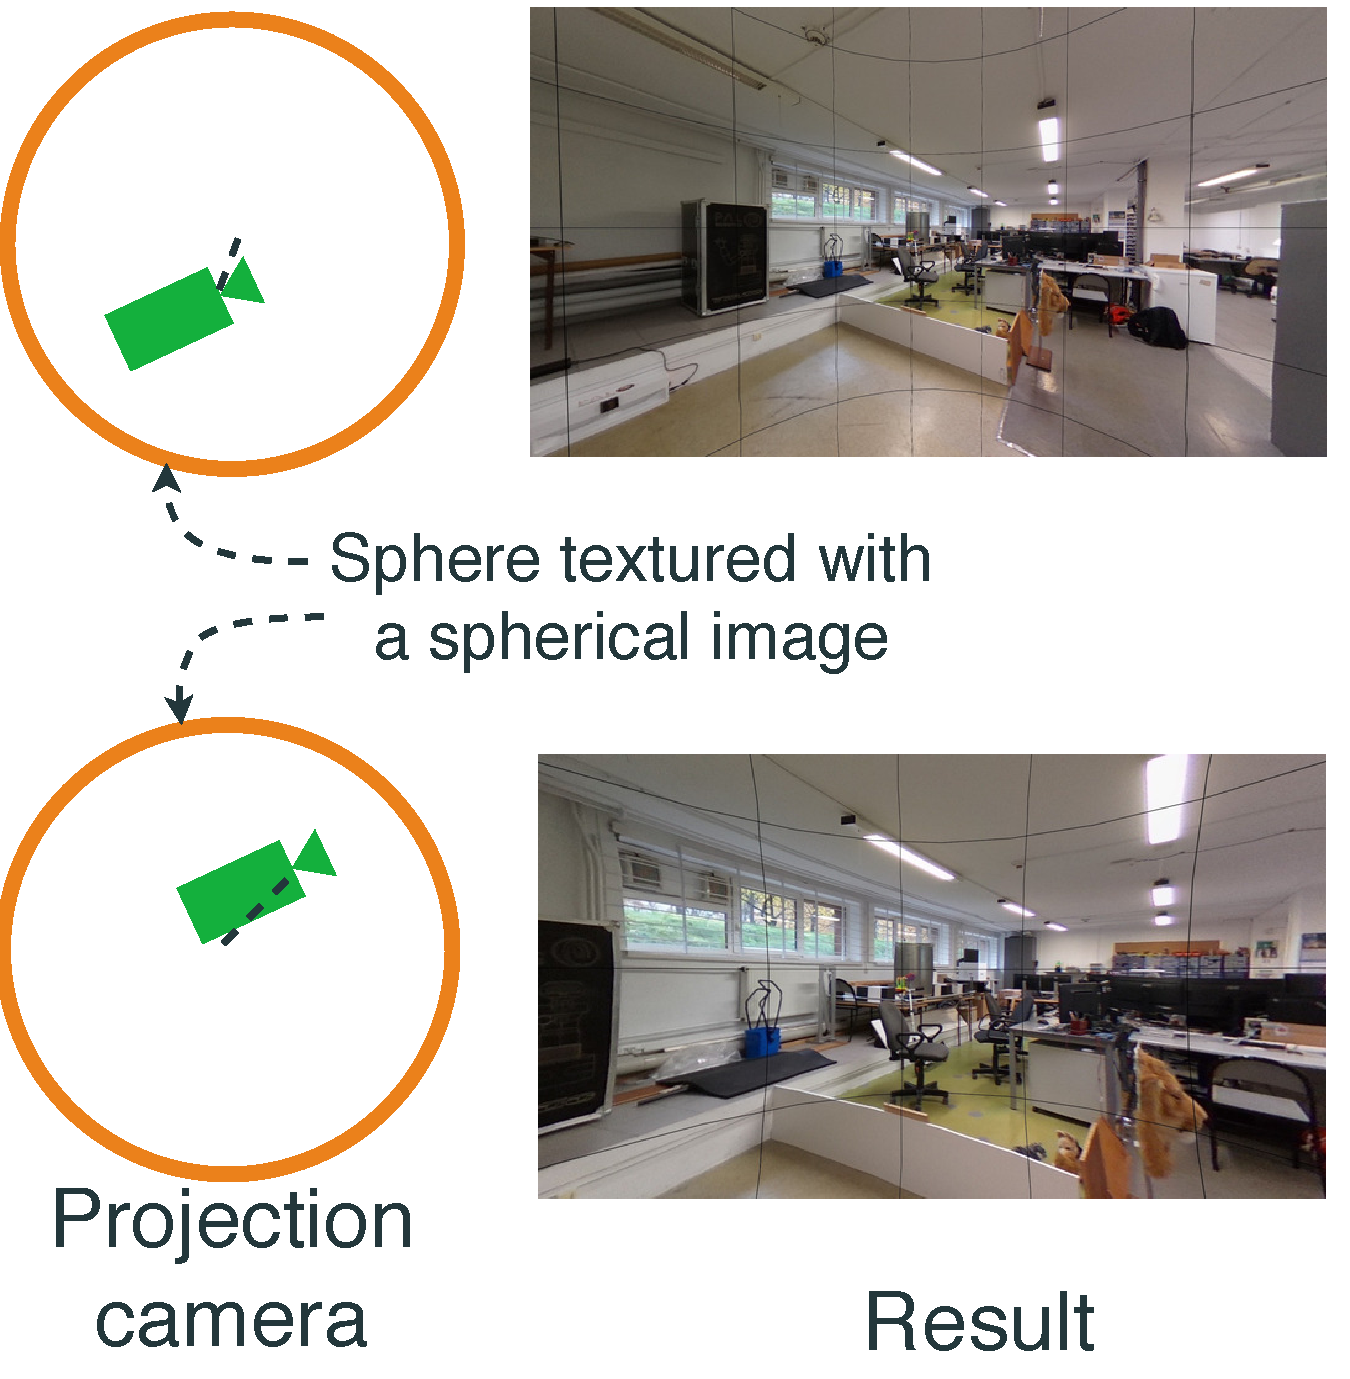
\includegraphics[width=0.45\textwidth]{img/interpolation/proj.pdf}
    \caption{Interpolation challenges: a) arrangement resulting in identical generated images; b) the method of interpolating camera views}
    \label{fig:interpolation}
\end{figure}

A simple solution to this problem would be to mimic the position of the virtual camera relative 
to a region with the position of the projection camera thus creating the ilusion of moving closer 
to certain objects as visualized in Fig.~\ref{fig:interpolation}b. This solution is not perfect,
as there will be no parallax visible, but with the photos sampled sufficiently dense the effect is satisfactory.

\todo[inline]{Można jeszcze dopisać kilka zdań o prefetchingu zdjęć (albo tutaj albo przy testach).}

\section{Gazebo integration}
\label{sec:gazebo}

So far, the robot is able to look around and move through the prepared environment. 
Generated images can be further processed in order to make this solution more versatile.
As the position and orientation of vierual camera is known, and its parameters are the same
as the projection camera, 3D view rendered in Gazebo can be overlaid onto the photo.
Fig. \ref{fig:join} depicts an example of such process.
In order to remove unwanted objects from the image additional plugin to the Gazebo simulator
was prepared to hide the objects from rendering in virtual camera, keeping them 
visible for other sensors (like laser scanner or sonars), thus keeping the obstacle avoidance
still working. This provides additional simulation features mentioned in the introduction. 
It enables the tester to modify the testing environment and provides the means of interaction 
of the simulated robot with the environment by the means of the Gazebo simulator.

\begin{figure}[!ht]
    \centering
        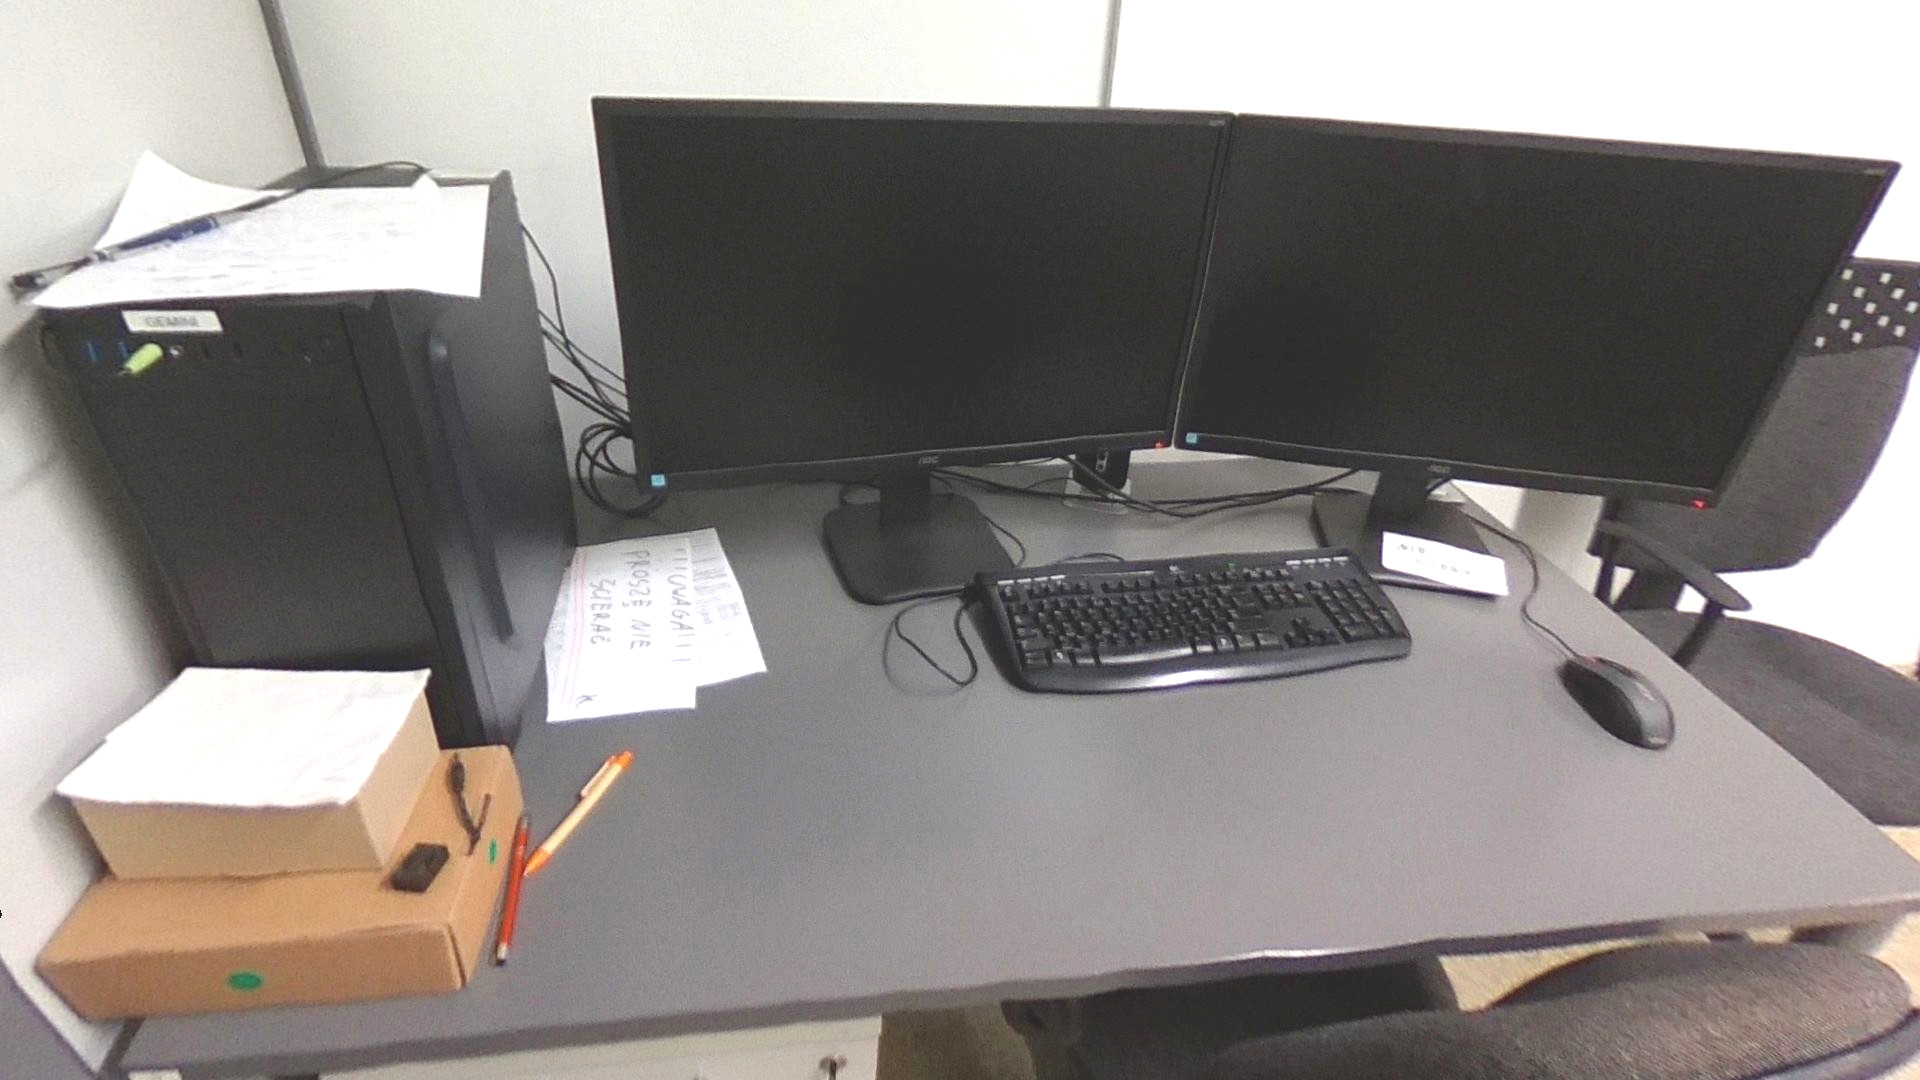
\includegraphics[width=0.33\textwidth,trim=29cm 2cm 0 10cm,clip]{img/gazebo_integration/sim.jpg}\hfill%
        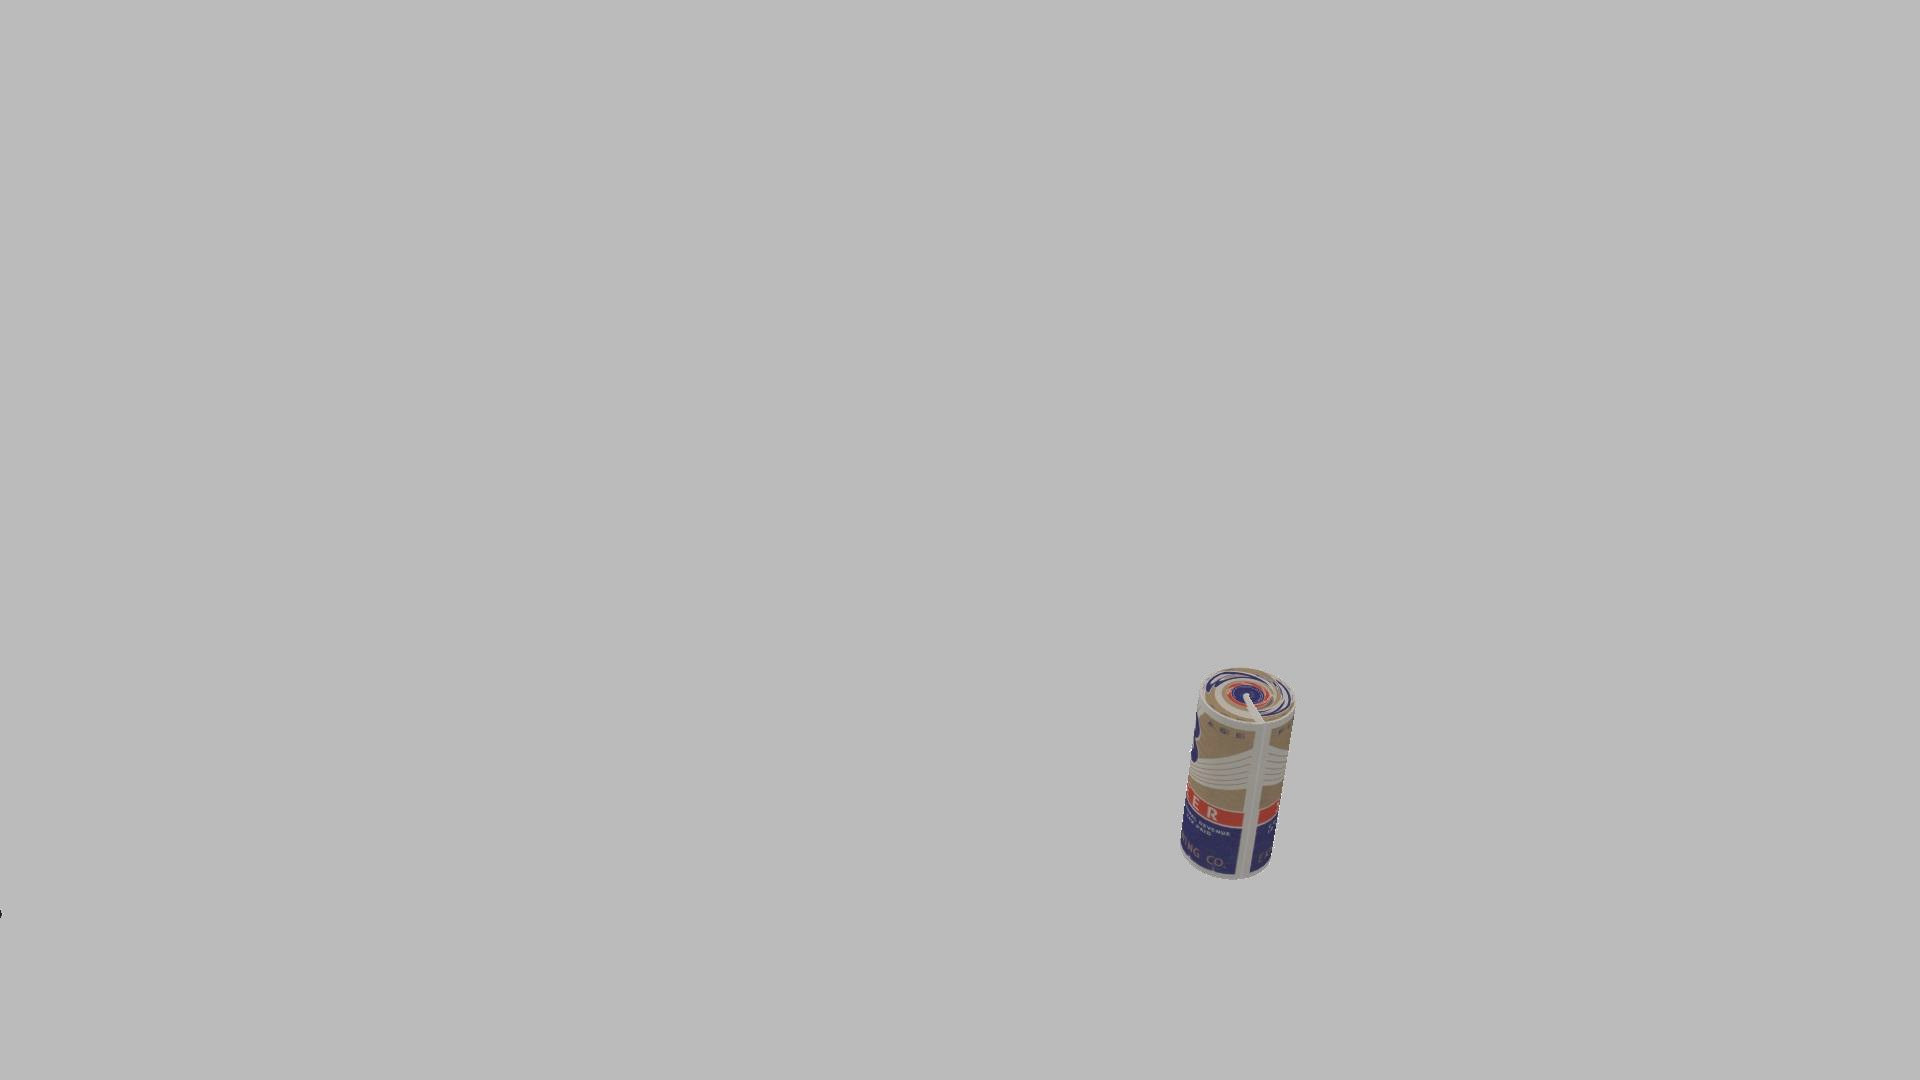
\includegraphics[width=0.33\textwidth,trim=29cm 2cm 0 10cm,clip]{img/gazebo_integration/gazebo.jpg}\hfill%
        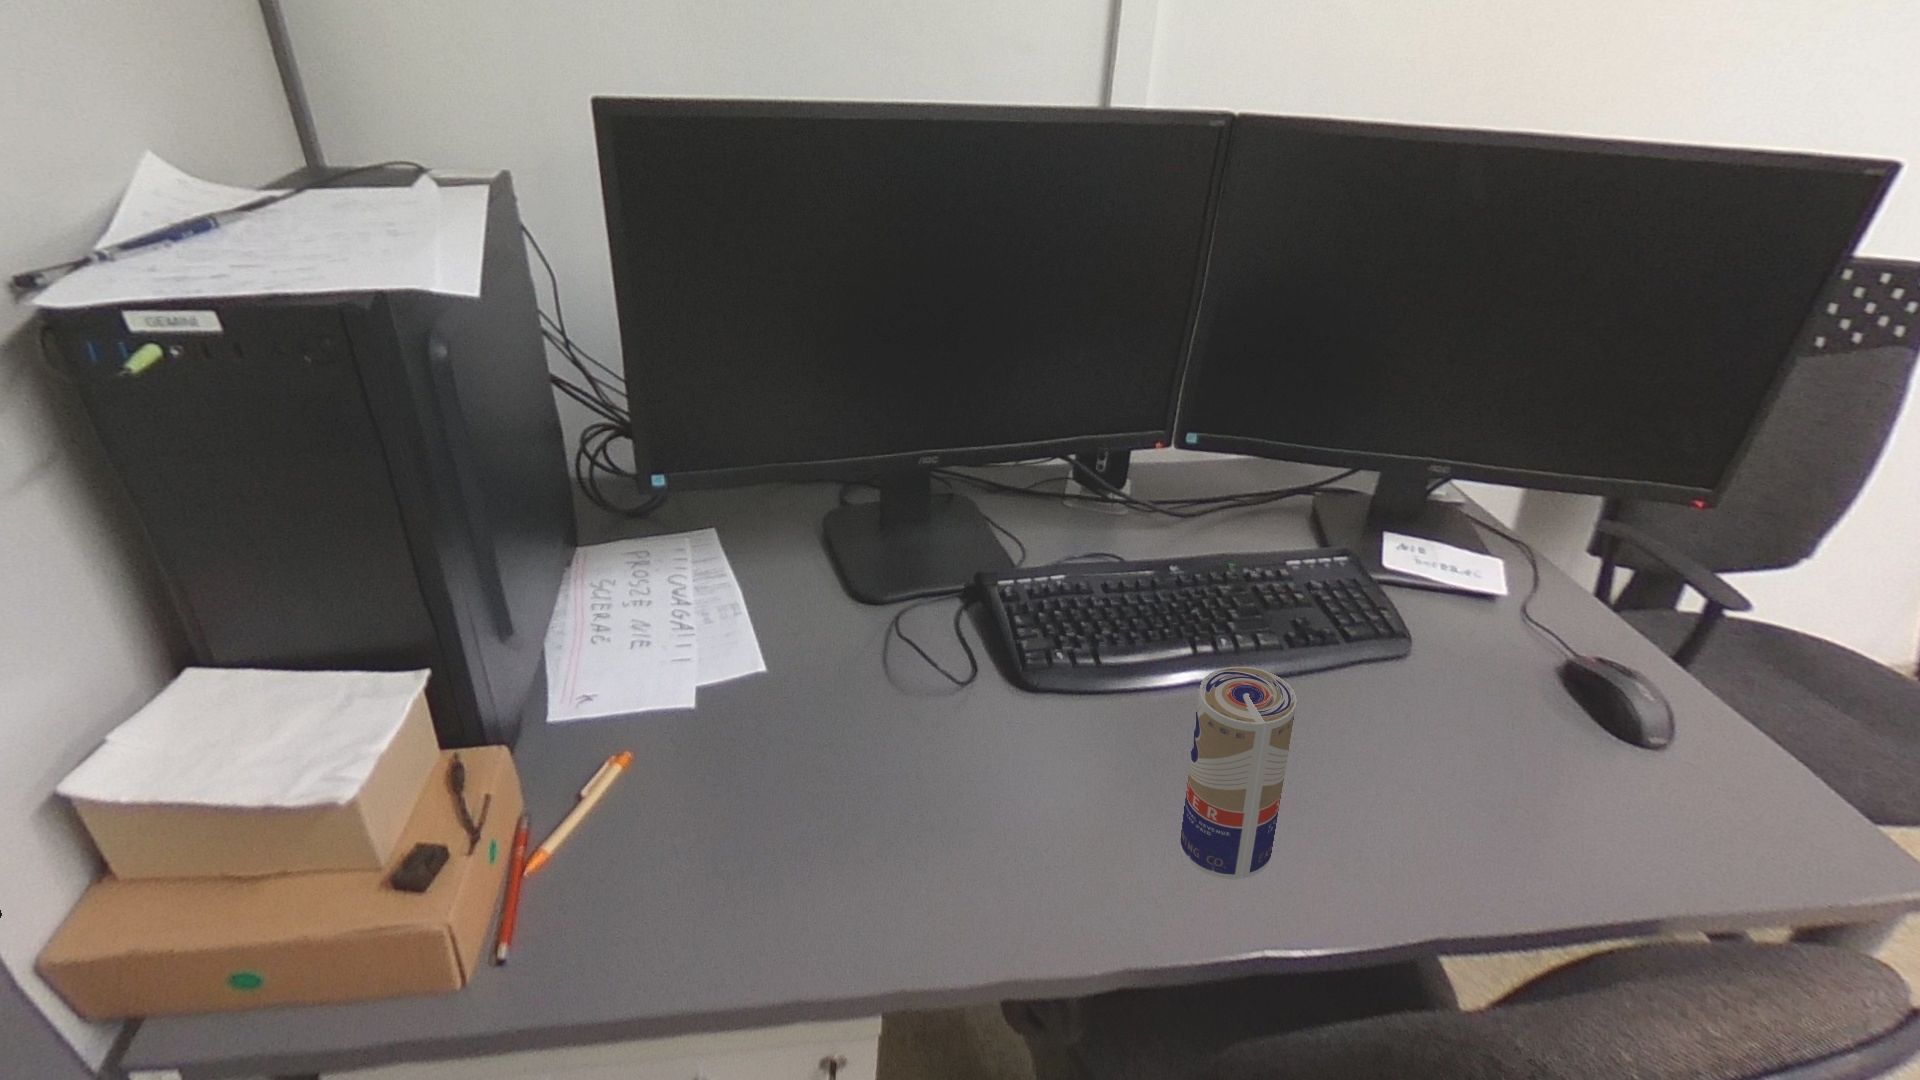
\includegraphics[width=0.33\textwidth,trim=29cm 2cm 0 10cm,clip]{img/gazebo_integration/sum.jpg}\\
        \hfill (a) \hfill\hfill (b) \hfill\hfill (c) \hfill~
    \caption{Adding virtual objects (b) to the generated images (a)}
    \label{fig:join}
    \vspace{-5mm}
\end{figure}


\section{Evaluation}
\label{sec:evaluation}

The simulation system presented above was tested in our robotics laboratory. At first individual modules
and system parameters were evaluated, followed by the partial scan of the room. Prepared environment is 
meant to be used with the Tiago robot, applied to service tasks related with elderly care and assistance.

\subsection{Camera selection}

In order to acquire full spherical photo, a dedicated camera setup is required. Nowadays, there are different 
possibilities to achieve that, without the need for building multiple camera rig from scratch. If the price 
doesn't matter, Ladybug5+ from Flir is the option. Its precalibrated 6 cameras provides 360\textdegree\ 
panorama with 8K resolution. On the consumer side of the market there are a few different devices to choose from,
most of them built from two fish-eye cameras facing in opposite directions. We chose the Theta V camera from Ricoh. 
This camera is capable of on-board image stitching to the equirectangular projection with final resolution
$5376\times2688$ pixels (created from two 4K photos). Another useful feature is possibility to capture
and transfer photos using WiFi. Average angular resolution of selected camera is around 15 px/\textdegree, 
which is more than the 10 px/\textdegree\ of a robots camera. 

\subsection{Rendering performance}

All the advantages of even the most advanced and photorealistic simulation are useless if its performance 
doesn't allow for (near)realtime work. There are to independent factors in photo rendering that can limit
the simulation performance. When the robot moves inside a single cell (in range of a single spherical
photo) only the rendering time is important. For our system it takes on average 0.365 ms to
render single VGA view. This allows us for simulating the camera with 2740 FPS. 

The other latency is a result of loading spherical photo from disk, decoding it and loading it into the memory of the video card.
A single 5376 $\times$ 2688 pixels JPEG image takes on average $t = 198.672\,ms$ to load and decode on our system.
This further limits the FPS to 5 if the images are loaded synchronously.
However, if the images can be loaded in advance, this would migitate the negative impact of the load latency on the robot's maximum speed.
In this case simulated robot's maximum speed $v_{max}$ depends on the amount of primary memory.

In order to achieve scaling $v_{max}$ with memory, one can utilise a pool of threads or processes.
In this case an important problem is choosing which spherical images should be cached in RAM.
The simplest strategy is to always store four images that were taken closest to the current position of the robot.
Such a solution often loads many images that will not be used for simulation.
A more sophisticated method would be to predict the movement of the robot.
For example, robot's velocity vector could be projected forward until it intersects the border of a cell.
Then, this image would be decoded and loaded in advance.

With just one thread or process for decoding images, the grid resolution of $20 cm$ and image load time of $200 ms$, the theoretical aggregated speed limit of the simulated robot is equal to $1\,\frac{m}{s}$.
According to TIAGo's datasheet \footnote{http://pal-robotics.com/wp-content/uploads/2019/07/Datasheet\_TIAGo\_Complete.pdf} this value coincides with real robot's maximum speed.

\subsection{Grid resolution and interpolation parameters}

Proper distance between consecutive photos is not easy to decide and depends on the
actual environment. Photos captured to sparce will result in big jumps when camera
moves between different grid points. Too dense and image loading and decoding
times will limit the speed of the robot in simulation to unacceptable values.

In order to make such a decision, first we created a relatively small but dense spherical photo set.
Then example images were generated for a given position and orientation of the virtual camera using that set.
Next we made the grid more sparse by selecting every second, third, fourth, etc. photo from the set and generated images for each step.
Some of the generated images can be seen on Fig. \ref{fig:grid_sizes}.
The grid resolution of 20 cm provided a good balance between the quality of the simulation and the time needed for the creation of the photo set.

\begin{figure}[!ht]
    \centering
    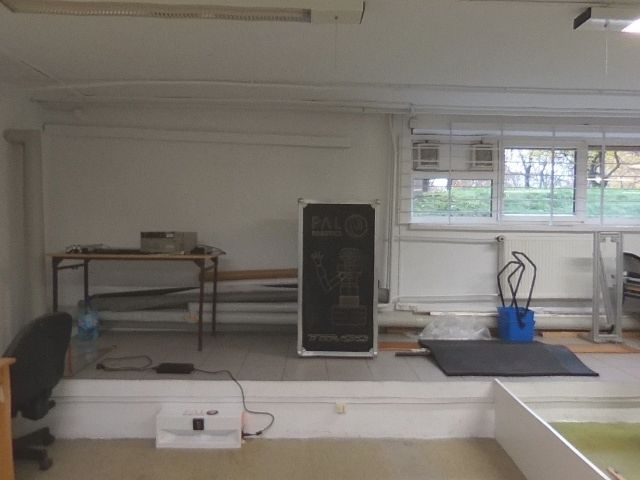
\includegraphics[width=0.33\textwidth]{img/grid_sizes/10}\hfill%
    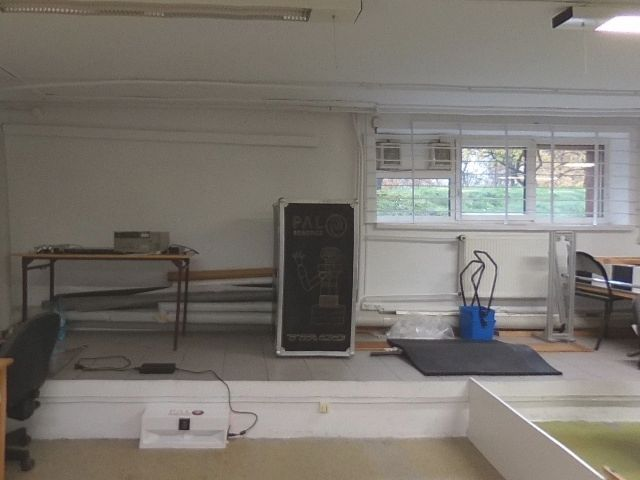
\includegraphics[width=0.33\textwidth]{img/grid_sizes/50}\hfill%
    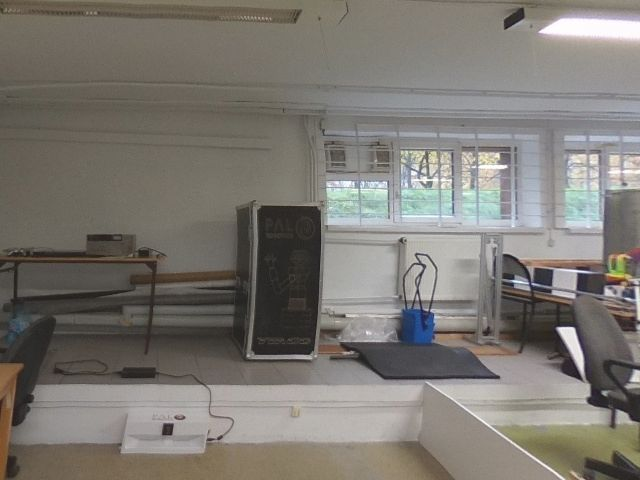
\includegraphics[width=0.33\textwidth]{img/grid_sizes/100}\\
    \caption{Example images generated with grid resolutions of 20, 100 and 200 cm.}
    \label{fig:grid_sizes}
\end{figure}

\subsection{Collecting photos of the target environment}

Finally, when all the parameters are selected, a set of spherical images can be created.
To facilitate the whole process we've created helper hardware and software.
For accurate photo capture and straight camera movement the device on Fig. \ref{fig:rig} was used.
It consists of a rail and a cart to which a monopod has been fixed.
At the other end of the monopod there is a mounting point for the camera.
A grid marks were put on the rail in order to allow precise positioning of the cart.
Similar marks were put on the floor in order to guide the rail.

\begin{figure}[!ht]
    \centering
    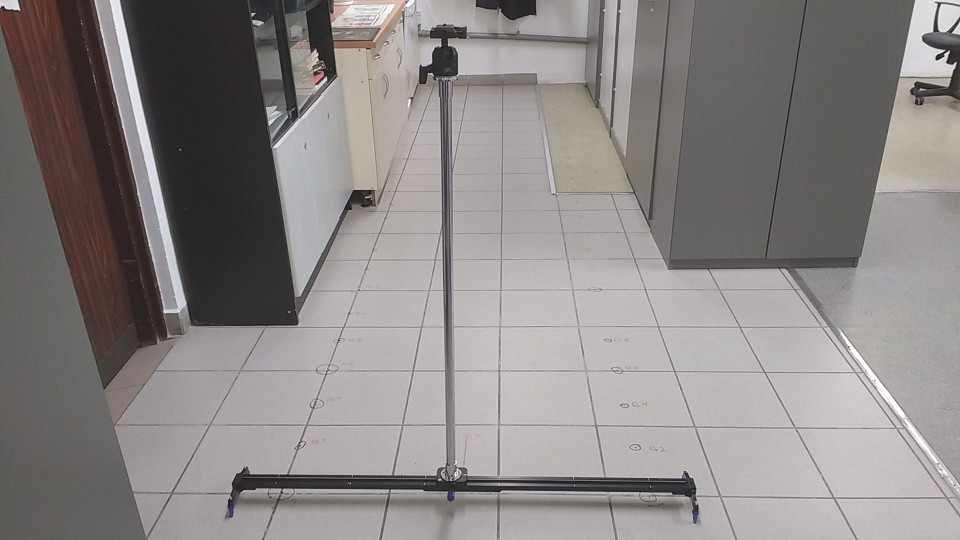
\includegraphics[width=0.49\textwidth]{img/rig/calosc.jpg}\hfill%
    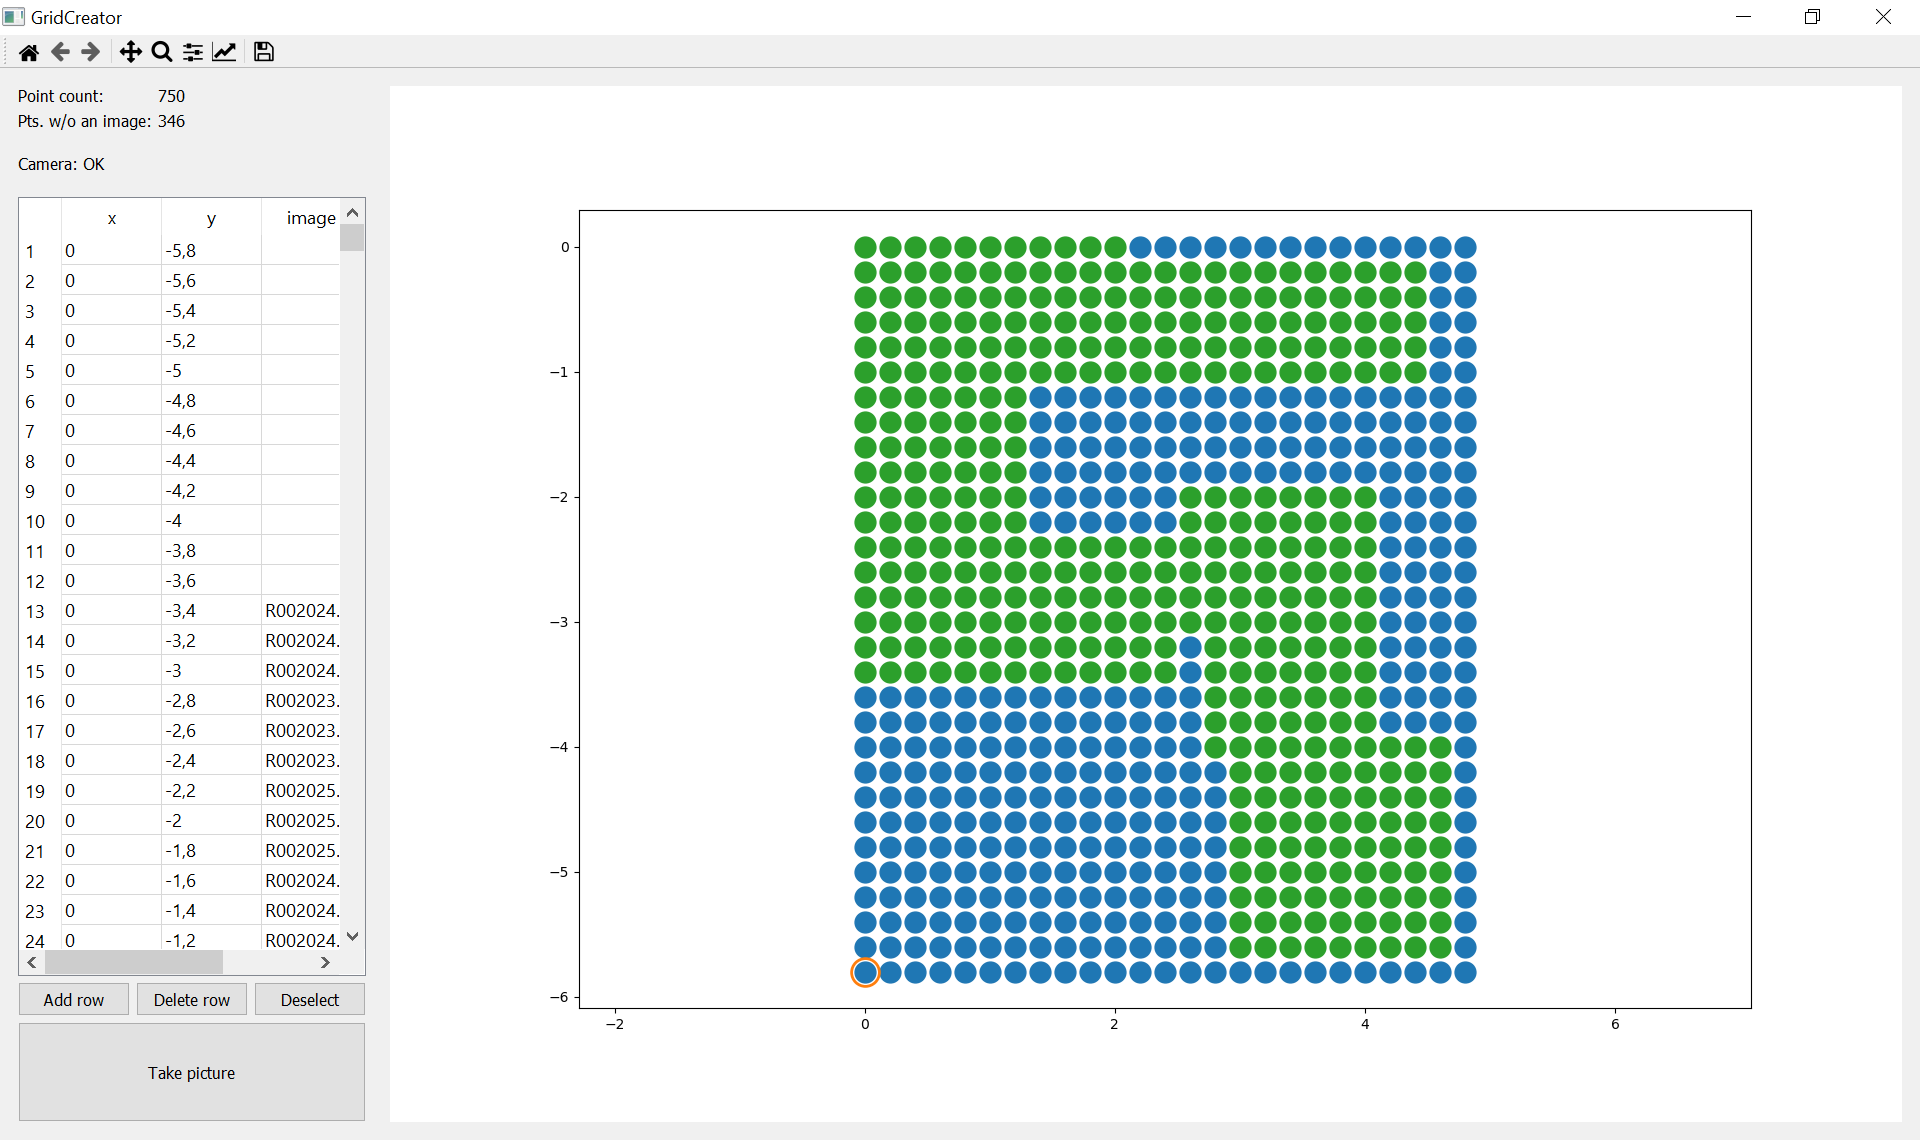
\includegraphics[width=0.49\textwidth]{img/creator.png}\\
    %\hfill (a) \hfill \hfill (b) \hfill ~\\
    \caption{Hardware and software used for the creation of the image set}
    \label{fig:rig}
\end{figure}

To simplify the process and keep track of photos that are already taken and still waiting to 
be captured, an application was created (Fig. \ref{fig:rig}).
It allows for selecting points and sending requests to the camera for taking pictures using the
Open Spherical Camera API. It also automatically tags the images with the correct position.

In the selected room, 404 pictures were taken in $20 cm$ intervals, covering the living room part,
the kitchen and part of the corridor. The whole process took 2 hours and 17 minutes,
which yields approximately 3 pictures taken per minute. 


The whole solution was evaluated by comparing generated images with images from a real robot.
For this purpose the TIAGo robot was used.
It was booted up and manually controlled in order to take pictures.
Then the proposed solution was used to generate images corresponding to pictures taken by TIAGo.
Finally, images from both sources were compared as seen on Fig. \ref{fig:sim_vs_tiago}.

\begin{figure}[!ht]
    \centering
    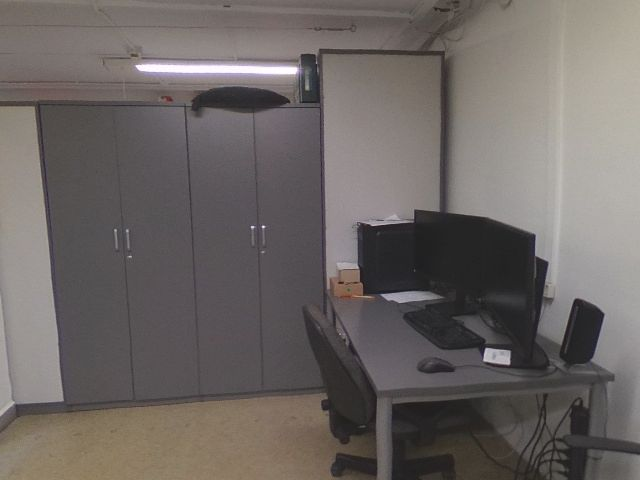
\includegraphics[width=0.33\textwidth]{img/sim_vs_tiago/sim_biurko.jpg}\hfill%
    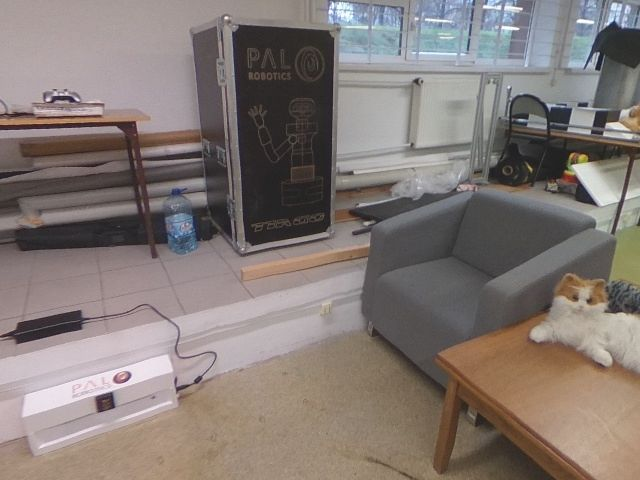
\includegraphics[width=0.33\textwidth]{img/sim_vs_tiago/sim_fotel.jpg}\hfill%
    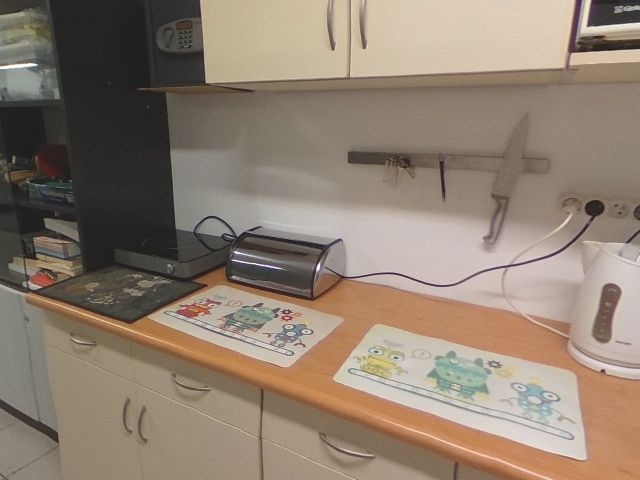
\includegraphics[width=0.33\textwidth]{img/sim_vs_tiago/sim_kuchnia_blat.jpg}\\
    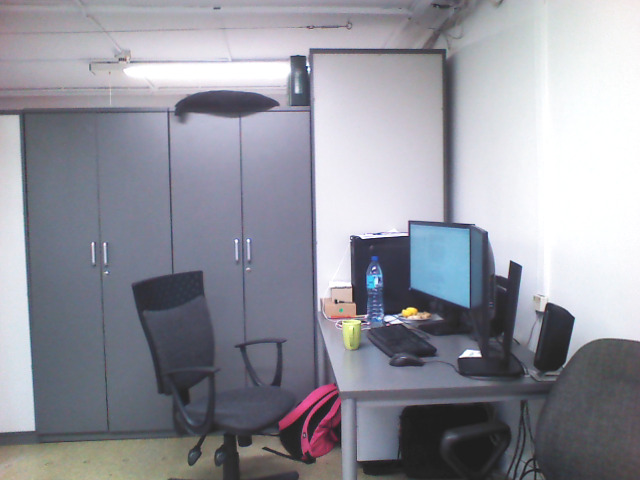
\includegraphics[width=0.33\textwidth]{img/sim_vs_tiago/tia_biurko.jpg}\hfill%
    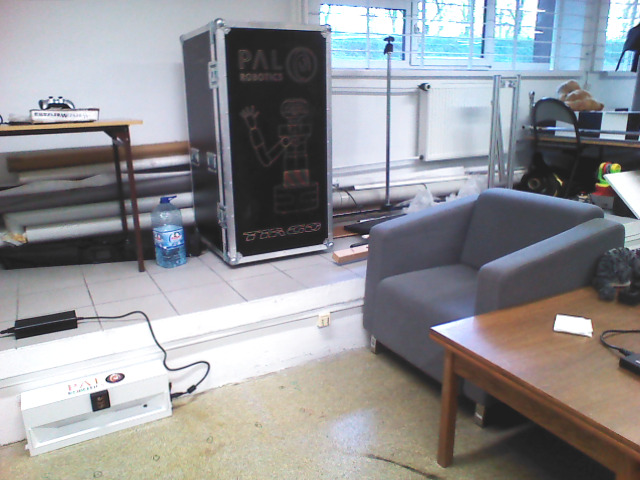
\includegraphics[width=0.33\textwidth]{img/sim_vs_tiago/tia_fotel.jpg}\hfill%
    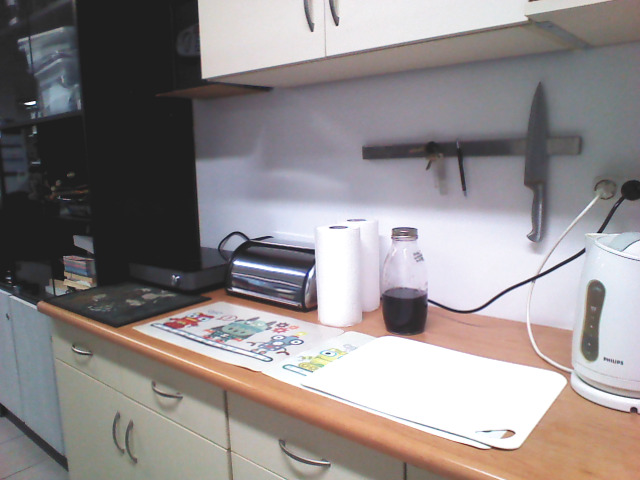
\includegraphics[width=0.33\textwidth]{img/sim_vs_tiago/tia_kuchnia_blat.jpg}\\
    \caption{Images generated in simulation (top) and taken by the robot (bottom)}
    \label{fig:sim_vs_tiago}
\end{figure}

\section{Conclusions}

The article presented the idea and exemplary application for the spherical camera based 
simulator for service robots. System was tested by comparing images generated in simulation
with those gathered by the real robot. The images differ mainly in color appearance 
and are otherwise nearly identical. The mentioned color issue can be resolved by the 
means of color correction. Those results prove that using the proposed solution a set 
of spherical images can be used to replace a real robot in software testing.

There are some issues in the system that can be improved. The process of photo acquisition
at the moment is highly manual labour. For each photo one has to move the camera, hide from
the camera view and gather a photo. In its current form it takes around 8 minutes per square meter.
The natural extension would be to utilize a robotic platform to move the camera around and
take photos automatically.

Manual photo capturing results also in slight misalignments between consecutive frames.
Photo stabilization techniques could be implemented to calculate angular offsets for each
image.

Created photo collection can also be extended with depth information calculated from multiview
structure estimation. This would make the interpolation process work better and allow for, 
possibly, grid with bigger steps.

\section*{Acknowledgments}
\label{sec:acknowledgments}
This work was funded within the INCARE AAL-2017-059 project "Integrated Solution for Innovative Elderly
Care" by the AAL JP and co-funded by the AAL JP countries.

\bibliographystyle{splncs03} 
\bibliography{bibliography}

\end{document}
